% Conceptual explainer for "Fairness Is Advantage-Neutral".
% Build: tectonic Fairness_Explained.tex
\documentclass[11pt,a4paper]{article}
\usepackage{amsmath,amsthm,amssymb}
\usepackage{newpxtext,newpxmath}
\usepackage[a4paper,margin=25mm]{geometry}
\usepackage{graphicx,booktabs,enumitem,xcolor,tikz}
\usetikzlibrary{arrows.meta,positioning,calc,shapes.geometric,decorations.pathmorphing}
\usepackage[colorlinks=true,linkcolor=black,citecolor=black,urlcolor=black]{hyperref}

\definecolor{agA}{HTML}{1F4E9A}
\definecolor{agB}{HTML}{A02020}
\definecolor{soft}{HTML}{F2F2F2}

\newcommand{\keyidea}[1]{%
  \par\smallskip\noindent\fcolorbox{black!40}{soft}{\parbox{\dimexpr\linewidth-2\fboxsep-2\fboxrule}{\small #1}}\par\smallskip}

\title{\textbf{Fair Allocation, Prices and Quantum Sampling}\\[3pt]
\large A conceptual guide to \emph{Fairness Is Advantage-Neutral}}
\author{Companion notes to the manuscript by Ritesh Roshan}
\date{}

\begin{document}
\maketitle

\begin{abstract}
\noindent This guide explains the whole project from the beginning, without assuming a background in
convex analysis, Markov chains or quantum computing. It follows one tiny example (three wireless links,
two users) from the question ``what is fair?'' to the quantum circuit, and at each step says what the
corresponding theorem in the manuscript does. Section~\ref{sec:known} separates what is new from
what was already known.
\end{abstract}

\tableofcontents
\bigskip

% ======================================================================
\section{The problem}

Some resources cannot be split. A transmission slot goes to one link or another, a ventilator to one
patient or another. When several people need them, we must decide who gets what, and we want the
decision to be \emph{fair} as well as efficient.

\paragraph{The running example.}
Three wireless links $a$, $b$, $c$ sit in a row. Neighbouring links interfere, so $a$ and $b$ cannot
transmit together, and neither can $b$ and $c$. Links $a$ and $c$ are far apart and can. User~1 owns
links $a$ and $c$; user~2 owns link $b$. Every link carries one unit of data when it transmits.

\begin{figure}[h]
\centering
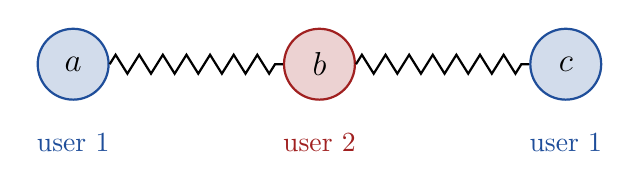
\begin{tikzpicture}[node distance=22mm,
  lk/.style={circle,draw,thick,minimum size=9mm,font=\large}]
\node[lk,fill=agA!20,draw=agA] (a) {$a$};
\node[lk,fill=agB!20,draw=agB,right=of a] (b) {$b$};
\node[lk,fill=agA!20,draw=agA,right=of b] (c) {$c$};
\draw[thick,decorate,decoration={zigzag,amplitude=1.2mm,segment length=3mm}] (a)--(b);
\draw[thick,decorate,decoration={zigzag,amplitude=1.2mm,segment length=3mm}] (b)--(c);
\node[below=3mm of a,agA] {user 1};
\node[below=3mm of b,agB] {user 2};
\node[below=3mm of c,agA] {user 1};
\end{tikzpicture}
\caption{The conflict graph of the running example. A jagged edge means ``cannot transmit at the same
time''.}
\label{fig:graph}
\end{figure}

\noindent A \emph{schedule} is a set of links that may transmit together: a set with no conflicting
pair, which graph theory calls an \emph{independent set}. There are five:
\[
\varnothing,\quad \{a\},\quad \{b\},\quad \{c\},\quad \{a,c\}.
\]
The two interesting ones are $\{a,c\}$, which gives user~1 two units and user~2 nothing, and $\{b\}$,
which gives user~1 nothing and user~2 one unit.

\keyidea{\textbf{The difficulty in one line.} Every single schedule leaves somebody with nothing.
No deterministic choice is fair.}

% ======================================================================
\section{What does ``fair'' mean?}

Economists have many answers, and the paper handles all of the standard ones~\cite{atkinson,rawls,nash,moulin}.
Write $y_1,y_2$ for what the two users receive.

\begin{center}\small
\begin{tabular}{@{}lll@{}}
\toprule
Criterion & Formula & Plain meaning\\
\midrule
Utilitarian & $y_1+y_2$ & maximise the total, ignore who gets it\\
Max-min (Rawls) & $\min(y_1,y_2)$ & make the worst-off person as well off as possible\\
Nash welfare & $\log y_1+\log y_2$ & balance total and equality (proportional fairness)\\
$\alpha$-fairness & $\sum_i y_i^{1-\alpha}/(1-\alpha)$ & a dial from utilitarian ($\alpha=0$) to max-min ($\alpha\to\infty$)\\
Gini-based welfare & mean $\times$ (1 $-$ Gini) & penalise inequality in the whole distribution\\
\bottomrule
\end{tabular}
\end{center}

\noindent All of these are \emph{concave}: spreading a fixed amount more evenly never lowers them.
That single property is all the theory needs. We use max-min as the running criterion because it is
the easiest to picture.

\subsection{Randomising: the lottery}
Since every schedule is unfair, use a lottery: pick $\{a,c\}$ with probability $p$ and $\{b\}$ otherwise.
On average user~1 gets $2p$ and user~2 gets $1-p$. These are equal when $p=\tfrac13$, and then each user
expects $\tfrac23$.

\keyidea{\textbf{Deterministic max-min value: $0$. Lottery max-min value: $\tfrac23$.}
This is \emph{ex-ante} fairness: fair in expectation, before the coin is tossed. Weighted lotteries are
already used to allocate scarce medicines~\cite{white,pathak}. If the allocation is repeated every time
slot, the long-run averages also approach $\tfrac23$ each.}

% ======================================================================
\section{Why fairness is awkward for quantum optimisers}

Quantum annealers and algorithms such as QAOA~\cite{qaoa,lucas} accept an objective that is a
\emph{quadratic} polynomial in yes/no variables $x_v\in\{0,1\}$ (``does link $v$ transmit?''). Many
fairness criteria are not quadratic. The minimum of $n$ yes/no variables equals their product
$x_1x_2\cdots x_n$, which has degree $n$, and an absolute value $|u_1-u_2|$, the building block of the
Gini coefficient, already has degree three in a small example. Forcing such a criterion into quadratic
form requires extra variables and penalty terms~\cite{boros}, which is why earlier quantum work on
equity either used a quadratic stand-in for fairness or left fairness out of the Hamiltonian.

\keyidea{\textbf{The paper's first observation:} this barrier exists only for single allocations. Once
we allow lotteries, the barrier disappears, as the next section shows.}

% ======================================================================
\section{The key idea: fairness is a set of prices}\label{sec:prices}

\subsection{The picture}
Plot each schedule as a point (what user~1 gets, what user~2 gets): $\{a,c\}\mapsto(2,0)$,
$\{b\}\mapsto(0,1)$, $\{a\},\{c\}\mapsto(1,0)$, $\varnothing\mapsto(0,0)$. A lottery produces an
\emph{average}, and averages of points fill in the shaded triangle of Figure~\ref{fig:hull}, the
\emph{convex hull}. The fairest lottery is the point of the triangle that is best for the chosen
criterion; for max-min it is where the diagonal $y_1=y_2$ leaves the triangle, at
$(\tfrac23,\tfrac23)$.

\begin{figure}[h]
\centering
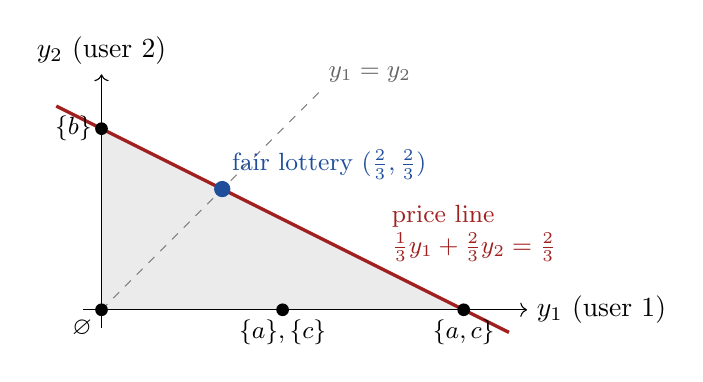
\begin{tikzpicture}[scale=2.3]
\fill[black!8] (0,0)--(2,0)--(0,1)--cycle;
\draw[->] (-0.1,0)--(2.35,0) node[right] {$y_1$ (user 1)};
\draw[->] (0,-0.1)--(0,1.3) node[above] {$y_2$ (user 2)};
\draw[dashed,black!50] (0,0)--(1.2,1.2) node[above right,black!60,font=\small] {$y_1=y_2$};
\draw[very thick,agB] (-0.25,1.125)--(2.25,-0.125);
\node[agB,font=\small,align=left,anchor=west] at (1.55,0.42) {price line\\ $\tfrac13 y_1+\tfrac23 y_2=\tfrac23$};
\foreach \p/\l/\pos in {{(2,0)}/{\{a,c\}}/below, {(0,1)}/{\{b\}}/left, {(1,0)}/{\{a\},\{c\}}/below, {(0,0)}/{\varnothing}/below left}
  \fill \p circle (0.035) node[\pos,font=\small] {$\l$};
\fill[agA] (2/3,2/3) circle (0.045) node[above right,agA,font=\small] {fair lottery $(\tfrac23,\tfrac23)$};
\end{tikzpicture}
\caption{Every lottery lands in the shaded triangle. The fair point is where the diagonal leaves it. The
red line, the ``price line'', touches the triangle exactly there and passes through the two schedules
that the fair lottery mixes.}
\label{fig:hull}
\end{figure}

\subsection{Prices}
Now give each user a \emph{priority weight}, or price, $\theta_i\ge0$ with $\theta_1+\theta_2=1$, and ask
a purely combinatorial question: \emph{which schedule has the largest priority-weighted value
$\theta_1y_1+\theta_2y_2$?} At $\theta=(\tfrac13,\tfrac23)$ the schedules $\{a,c\}$ and $\{b\}$ tie at
$\tfrac23$, which is exactly the fair value. That is not a coincidence:

\keyidea{\textbf{Separation theorem (Theorem 2 of the paper).} For any concave fairness criterion,
\[
\underbrace{\max_{\text{lotteries}}\ \text{fairness}}_{\text{normative question}}
\;=\;\min_{\text{prices }\theta}\Bigl[\;\underbrace{\max_{\text{schedules }x}\ \theta\cdot u(x)}_{\text{combinatorial question}}
\;-\;\underbrace{\Psi_*(\theta)}_{\text{penalty set by the criterion}}\Bigr].
\]
For max-min the penalty is zero and the prices range over all weights summing to one.
The \emph{fairness criterion} only says which prices are allowed. The \emph{feasible schedules} only
enter through the question ``what is the best schedule at these prices?''.}

\noindent The mathematics is classical convex duality, the same duality that turns a constrained
problem into a Lagrangian with multipliers~\cite{rockafellar,boyd}. The contribution is the reading:
the normative part (what is fair) and the combinatorial part (what is feasible) separate cleanly.

\paragraph{The SVM analogy.} A support vector machine finds a maximum-margin line, and at the optimum only
the \emph{support vectors}, the points touching the margin, carry nonzero dual weight. Here, at the
optimum only the \emph{worst-off users} carry nonzero price. In the example both users are worst-off
together, so both prices are positive, and the price line touches the triangle at the two schedules the
fair lottery mixes.

\subsection{Two consequences}
\begin{enumerate}[leftmargin=*]
\item \textbf{No representation cost (Corollary 3).} The question ``best schedule at prices $\theta$''
is a \emph{weighted} version of the usual problem, and it has the same polynomial degree as the
utilities. In scheduling it is the maximum-weight independent set problem, which is quadratic and native
to quantum hardware. Fairness never has to be written into the Hamiltonian at all.
\item \textbf{Advantage neutrality (Theorem 4).} Since fair allocation reduces to repeatedly solving the
weighted problem, and the weighted problem is itself a special case of fair allocation, the two are
equally hard on \emph{any} computer, classical or quantum. Fairness therefore cannot be the source of a
quantum speedup. If a quantum computer helps, it helps with the underlying combinatorial problem.
\end{enumerate}

% ======================================================================
\section{Doing it over time: priorities that learn}

We usually do not know the fair prices in advance. The paper finds them by \emph{learning} them while
allocating, round after round, with the multiplicative-weights (Hedge) rule~\cite{freundschapire,ahk}:

\keyidea{\textbf{The update.} After each round, multiply each user's priority by $e^{-\eta\,\cdot\,\text{what
they received}}$, then rescale so the priorities sum to one. Users who received a lot lose priority;
users who received little gain it.}

\noindent Here is the loop on the running example, with $\eta=0.5$ and, for now, each round simply
taking the best schedule at the current prices.

\begin{center}\small
\begin{tabular}{@{}cccccc@{}}
\toprule
Round & Priorities $(\theta_1,\theta_2)$ & Best schedule & Received & Running average & Worst-off average\\
\midrule
1 & (0.50, 0.50) & $\{a,c\}$ & (2, 0) & (2.00, 0.00) & 0.00\\
2 & (0.27, 0.73) & $\{b\}$ & (0, 1) & (1.00, 0.50) & 0.50\\
3 & (0.38, 0.62) & $\{a,c\}$ & (2, 0) & (1.33, 0.33) & 0.33\\
4 & (0.18, 0.82) & $\{b\}$ & (0, 1) & (1.00, 0.50) & 0.50\\
5 & (0.27, 0.73) & $\{b\}$ & (0, 1) & (0.80, 0.60) & 0.60\\
6 & (0.38, 0.62) & $\{a,c\}$ & (2, 0) & (1.00, 0.50) & 0.50\\
7 & (0.18, 0.82) & $\{b\}$ & (0, 1) & (0.86, 0.57) & 0.57\\
8 & (0.27, 0.73) & $\{b\}$ & (0, 1) & (0.75, 0.62) & 0.62\\
\bottomrule
\end{tabular}
\end{center}

\noindent From round 3 on, the priorities cycle around the fair price $\theta_1=\tfrac13$, and the
schedules settle into the pattern $\{a,c\},\{b\},\{b\}$, which is exactly the fair lottery
($\tfrac13$ and $\tfrac23$). The worst-off average climbs toward $\tfrac23$. Nobody told the algorithm
the answer; it was discovered by the priorities.

\paragraph{The Grover analogy.} Grover's search repeats two simple moves: flip the sign of the target,
then reflect every amplitude about the mean. The fairness loop repeats two simple moves: pick a schedule
at the current prices, then lower the priority of users who did better than average and raise it for
those who did worse. In both, one simple step is repeated, and the repetition does
the work.

\keyidea{\textbf{Regret guarantee (Theorem 9).} After $T$ rounds, the worst-off user's average is at
least the best achievable value minus an error that shrinks like $1/\sqrt{T}$, plus two small terms
explained next.}

% ======================================================================
\section{From ``best schedule'' to ``random good schedule''}

Finding the single best schedule at given prices is itself a hard problem in large networks (maximum
weight independent set is NP-hard). The paper therefore replaces ``take the best'' by ``draw a random
schedule that is \emph{probably} good'', using the Gibbs, or Boltzmann, distribution from physics:
\[
\Pr(\text{schedule } x)\;\propto\;e^{\,\beta\,\times\,\text{priority-weighted value of }x}.
\]
The dial $\beta$ is an inverse temperature. At $\beta=0$ every schedule is equally likely; as
$\beta\to\infty$ only the best one survives. At the fair price $\theta=(\tfrac13,\tfrac23)$ with $\beta=3$
the example gives:
\begin{center}\small
\begin{tabular}{@{}lccccc@{}}
\toprule
Schedule & $\varnothing$ & $\{a\}$ & $\{c\}$ & $\{b\}$ & $\{a,c\}$\\
Probability & 0.8\% & 5.9\% & 5.9\% & 43.7\% & 43.7\%\\
\bottomrule
\end{tabular}
\end{center}
The two tight schedules dominate, and weak ones still appear occasionally. The price of this softness is
a small, known loss in fairness, the $\log|F|/(\beta n)$ term of Theorem 9 (Lemma 7); raising $\beta$
shrinks it.

\paragraph{Why sample at all?} Sampling is far easier than exact optimisation, and among all lotteries
with a given average the Gibbs lottery is the most random, or maximum-entropy, one (Theorem 8). It commits
to nothing beyond what fairness requires.

% ======================================================================
\section{How to draw a random schedule: Markov chains}

Listing all schedules is impossible in large networks, so the paper draws a sample with a random walk,
the Metropolis rule~\cite{metropolis,hastings}:

\begin{enumerate}[leftmargin=*]
\item From the current schedule $y$, \textbf{propose} a new schedule $x$, for example by switching one
link on or off.
\item If $x$ breaks an interference rule, stay at $y$.
\item If $x$ is more valuable, \textbf{move} to $x$. If it is less valuable, move with probability
$e^{\beta\times(\text{value}(x)-\text{value}(y))}$, otherwise stay.
\end{enumerate}

\noindent Repeated long enough, the walk visits each schedule with exactly its Gibbs probability. The
only requirement on the proposal is \emph{symmetry}: proposing $y\to x$ must be exactly as likely as
proposing $x\to y$.

\paragraph{How long is ``long enough''? The spectral gap.} Think of shuffling a deck. Moving one card at a
time takes thousands of moves to randomise it; a riffle shuffle takes about seven. The speed at which a
random walk forgets where it started is measured by one number, the \emph{spectral gap} $\gamma$: roughly
$1/\gamma$ steps are needed~\cite{levinperes}. Single-link flips are the ``one card at a time'' shuffle.
They get stuck when good schedules are far apart, as $\{a,c\}$ and $\{b\}$ are: going from one to the
other requires passing through worse schedules.

\keyidea{\textbf{Warm-start theorem (Theorem 11).} Priorities change only slightly per round, so the
target distribution changes only slightly, and the walk never has to start from scratch. Each round
needs about $\frac1\gamma\log\frac1\varepsilon$ steps, \emph{independent of the number of schedules}.
Hence the cost of fair allocation is governed by one number, the spectral gap $\gamma$ of the proposal,
and improving the proposal is the only place where a quantum computer can help.}

% ======================================================================
\section{Where the quantum computer enters}

\subsection{Rydberg atoms already know the rules}
In a Rydberg atom array, each atom is one link. An atom in its excited (Rydberg) state means ``this link
transmits''. Two excited atoms that are too close repel so strongly that the state cannot be reached:
the \emph{Rydberg blockade}~\cite{jaksch,bernien,ebadi}. If atoms are placed so that ``too close'' means
``interfering'', the hardware physically cannot produce an infeasible schedule.

\begin{figure}[h]
\centering
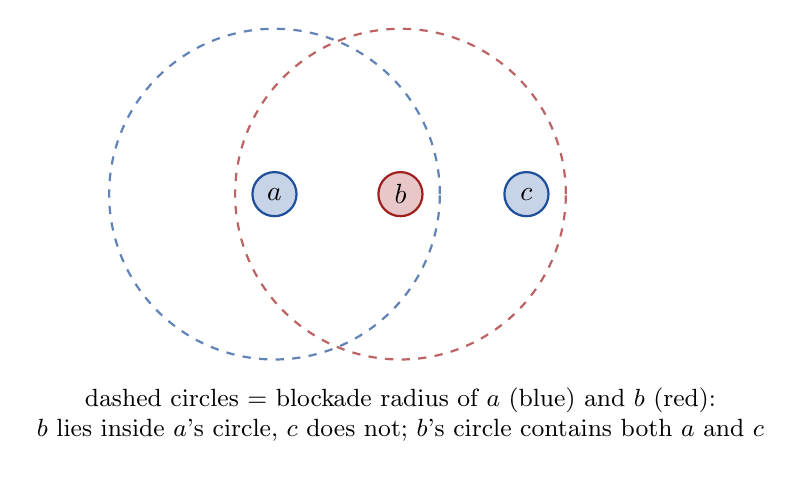
\begin{tikzpicture}
\draw[dashed,agA!70,thick] (0,0) circle (2.1);
\draw[dashed,agB!70,thick] (1.6,0) circle (2.1);
\foreach \x/\n/\col in {0/a/agA,1.6/b/agB,3.2/c/agA}{
  \fill[\col!25,draw=\col,thick] (\x,0) circle (0.28);
  \node at (\x,0) {$\n$};}
\node[font=\small,align=center] at (1.6,-2.8) {dashed circles = blockade radius of $a$ (blue) and $b$ (red):\\
$b$ lies inside $a$'s circle, $c$ does not; $b$'s circle contains both $a$ and $c$};
\end{tikzpicture}
\caption{The conflict graph of Figure~\ref{fig:graph} laid out as atoms. Blockade enforces the
interference rules for free.}
\end{figure}

\subsection{The quantum proposal}
Instead of flipping one link, the proposal lets the atoms evolve for a short time under two effects: a
\emph{driver} (the PXP Hamiltonian~\cite{turner}) that tries to switch each link on or off, but only if
all its neighbours are off, and a \emph{cost} term that makes valuable schedules gain phase. Measuring the
atoms gives the proposed schedule. Three facts make it exactly correct:

\begin{enumerate}[leftmargin=*]
\item \textbf{Never infeasible (Lemma 12).} Every step respects blockade, so the quantum state stays
inside the set of valid schedules.
\item \textbf{Exactly symmetric (Lemma 14).} The evolution is built as a palindrome, running forwards
then mirror-image backwards within each step, from real symmetric pieces. Such a product equals its
own transpose, so ``$y\to x$'' and ``$x\to y$'' have exactly the same probability, at any circuit
depth.
\item \textbf{Exact target (Theorem 15).} A symmetric proposal inside the Metropolis rule gives exactly
the fair Gibbs lottery in the long run, whatever the quantum device does in between.
\end{enumerate}

\keyidea{\textbf{Intuition.} The quantum evolution is a riffle shuffle of schedules that can jump between
distant good schedules, such as $\{a,c\}$ and $\{b\}$, in one proposal, while the classical
accept/reject coin keeps the answer exactly right. The quantum part only needs to propose well; it never
has to be trusted to compute the answer.}

\noindent The paper also gives the gate-level circuit, with exact gate counts, for devices without
native blockade, and checks it against exact simulation to about $10^{-15}$.

% ======================================================================
\clearpage
\section{The whole algorithm on one page}

\begin{figure}[!h]
\centering
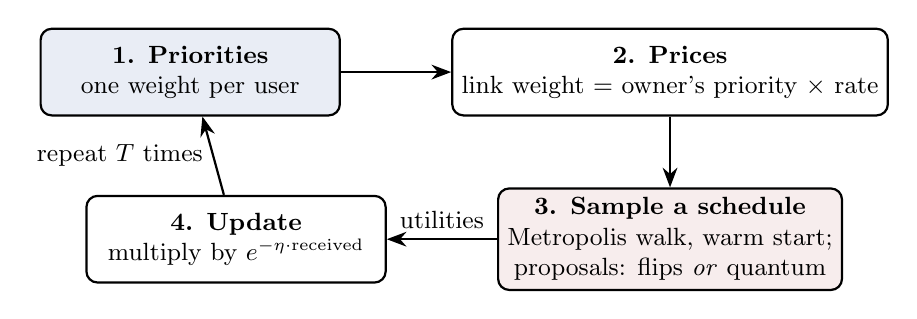
\begin{tikzpicture}[node distance=9mm and 14mm,
  box/.style={draw,thick,rounded corners,align=center,minimum width=38mm,minimum height=11mm,font=\small},
  ar/.style={-{Stealth[length=2.5mm]},thick}]
\node[box,fill=agA!10] (pri) {\textbf{1. Priorities}\\ one weight per user};
\node[box,right=of pri] (pr) {\textbf{2. Prices}\\ link weight = owner's priority $\times$ rate};
\node[box,below=of pr,fill=agB!8] (smp) {\textbf{3. Sample a schedule}\\ Metropolis walk, warm start;\\ proposals: flips \emph{or} quantum};
\node[box,left=of smp] (upd) {\textbf{4. Update}\\ multiply by $e^{-\eta\cdot\text{received}}$};
\draw[ar] (pri)--(pr);
\draw[ar] (pr)--(smp);
\draw[ar] (smp)--node[above,font=\small]{utilities} (upd);
\draw[ar] (upd)--node[left,font=\small]{repeat $T$ times} (pri);
\end{tikzpicture}
\caption{The fairness loop. Fairness lives in steps 1, 2 and 4; the quantum device lives only in step 3.}
\end{figure}

\begin{enumerate}[leftmargin=*]
\item Start with equal priorities.
\item Turn priorities into link weights.
\item Take a few Metropolis steps from the previous schedule, mixing local flips with quantum proposals;
the current state is this round's schedule.
\item Update priorities: whoever received less gains priority.
\item Repeat. The average allocation approaches the fairest lottery.
\end{enumerate}

\paragraph{What this algorithm is called.} There is no single established name, and the paper calls it
guided quantum Gibbs dynamics. In standard terms the outer loop is \emph{multiplicative weights} (Hedge),
a no-regret, primal--dual method that solves the zero-sum game between ``fairness'' and
``allocation''~\cite{freundschapire}. The inner loop is \emph{Metropolis--Hastings MCMC} with a
\emph{quantum-enhanced proposal}~\cite{layden}. The closest classical relative is adaptive CSMA in
wireless networks~\cite{jiangwalrand}.

% ======================================================================
\section{What the experiments show}

All numbers come from exact computation on networks of 8 to 20 links, in three families: unit-disk
graphs (geometric, like real radio networks), Erd\H{o}s--R\'enyi random graphs (dense) and random
3-regular graphs (sparse).

\begin{itemize}[leftmargin=*]
\item \textbf{Faster mixing, always.} The quantum proposal increases the spectral gap over single flips
in every instance, by factors of 3.4 to about 1100, with typical (geometric-mean) factors of 20 to 49 per
family.
\item \textbf{Better scaling, sometimes.} On dense random graphs the gap shrinks with network size about
half as fast as for the best classical proposal. On unit-disk graphs this holds only at high
temperature, and on sparse 3-regular graphs a classical swap move scales better.
\item \textbf{Fewer steps per round.} Along real fairness trajectories, the quantum proposal needs the
fewest steps in 82\% of 39 instances: 21 steps on average, against 32 for an idealised uniform proposal
and about 1900 for single flips.
\item \textbf{Fairer outcomes at equal effort.} In a 1500-round max-min run on a 12-link network, the
quantum-mixed chain reached a worst-off average of $1.327\pm0.007$ against $1.179\pm0.139$ classically,
with the best possible value $1.460$. It was also nineteen times more consistent from run to run.
\end{itemize}

\keyidea{\textbf{Honest summary.} These are large constant-factor gains and instance-dependent scaling
gains at small sizes. They are \emph{not} evidence of a general quantum advantage, and the paper says so.
Known limits apply: quantum proposals cannot help on unstructured problems~\cite{orfisels}, classical
solvers are strong on unit-disk graphs~\cite{andrist}, and a quantum step costs more time than a
classical flip.}

% ======================================================================
\section{What is new and what was already known}\label{sec:known}

\begin{center}\small
\begin{tabular}{@{}p{0.34\linewidth}p{0.6\linewidth}@{}}
\toprule
Already known & Where\\
\midrule
Concave fairness criteria and their duals & welfare economics, convex analysis~\cite{atkinson,rockafellar}\\
Max-min fair lotteries via repeated weighted welfare & Kawase and Sumita~\cite{kawasesumita}\\
Gibbs sampling of schedules with dual weights & adaptive CSMA~\cite{jiangwalrand}\\
Chains tracking slowly changing weights & network adiabatic theorem~\cite{rss}\\
Quantum proposals inside Metropolis & quantum-enhanced MCMC~\cite{layden}\\
Rydberg sampling of independent-set Gibbs states & Wild et al., by slow adiabatic preparation~\cite{wild}\\
\midrule
\textbf{New in this project} & \\
\midrule
\multicolumn{2}{@{}p{0.96\linewidth}@{}}{%
\begin{itemize}[leftmargin=*,nosep]
\item The separation theorem for \emph{every} concave criterion, and its consequence that fairness is
advantage-neutral: it cannot create or destroy a quantum speedup.
\item An explicit warm-start bound whose cost does not grow with the number of schedules.
\item A quantum proposal that is feasible by physics and exactly symmetric by construction at any depth,
given down to the gate level, used for the first time inside a fairness-driven sampler.
\item An open, verified implementation with exact benchmarks.
\end{itemize}}\\
\bottomrule
\end{tabular}
\end{center}

% ======================================================================
\section{Open questions}

\begin{enumerate}[leftmargin=*]
\item \textbf{One formula for the total cost.} Combining Theorems 9 and 11 should give ``total steps
$\approx$ (rounds needed for fairness) $\times$ (steps per round) $\approx \frac{\rho^2\ln n}{\varepsilon^2}\cdot\frac1\gamma\log\frac1\varepsilon$'',
making ``the spectral gap is everything'' a single theorem.
\item \textbf{When does quantum help?} Sampling independent sets is classically hard only above a sharp
threshold of the weights, the uniqueness threshold~\cite{sly}. Does the quantum gain switch on exactly
there? A single sweep across the threshold would answer it.
\item \textbf{Noise.} Real hardware breaks the exact symmetry slightly. How much bias does that cause? A
standard perturbation bound suggests about (asymmetry)$/\gamma$.
\item \textbf{Scale and fair baselines.} Larger networks (30--40 links) with stronger classical
competitors, such as parallel tempering and quantum-inspired proposals.
\end{enumerate}

% ======================================================================
\section*{Glossary}
\begin{description}[leftmargin=0pt,itemsep=2pt,font=\normalfont\bfseries]
\item[Independent set.] A set of links with no two in conflict; a valid schedule.
\item[Lottery (ex-ante).] A probability distribution over schedules; fairness judged on averages.
\item[Concave criterion.] A fairness score that never decreases when outcomes are spread more evenly.
\item[Convex hull.] All averages of a set of points; the set of outcomes lotteries can achieve.
\item[Prices / dual weights $\theta$.] Priority weights on users; the fairness criterion decides which are allowed.
\item[Weighted welfare.] $\sum_i\theta_iy_i$; the only question the combinatorial part ever answers.
\item[Multiplicative weights (Hedge).] Update rule that raises the priority of users who received little.
\item[Gibbs distribution, $\beta$.] Lottery with probability $\propto e^{\beta\cdot\text{value}}$; $\beta$ sets how greedy it is.
\item[Metropolis rule.] Propose a move, accept with probability $\min\{1,e^{\beta\Delta\text{value}}\}$.
\item[Spectral gap $\gamma$.] Mixing speed of a random walk; about $1/\gamma$ steps to forget the start.
\item[Rydberg blockade.] Nearby excited atoms are forbidden, so the hardware enforces conflicts.
\item[PXP driver.] Switches an atom only if all its neighbours are off.
\item[Palindromic Trotter step.] A product of gates that reads the same forwards and backwards; it makes
the proposal exactly symmetric.
\end{description}

% ======================================================================
\begin{thebibliography}{99}\small
\bibitem{andrist} Andrist RS et al. (2023) Hardness of the maximum-independent-set problem on unit-disk graphs and prospects for quantum speedups. Phys Rev Res 5:043277
\bibitem{ahk} Arora S, Hazan E, Kale S (2012) The multiplicative weights update method: a meta-algorithm and applications. Theory Comput 8:121--164
\bibitem{atkinson} Atkinson AB (1970) On the measurement of inequality. J Econ Theory 2:244--263
\bibitem{bernien} Bernien H et al. (2017) Probing many-body dynamics on a 51-atom quantum simulator. Nature 551:579--584
\bibitem{boros} Boros E, Hammer PL (2002) Pseudo-Boolean optimization. Discrete Appl Math 123:155--225
\bibitem{boyd} Boyd S, Vandenberghe L (2004) Convex Optimization. Cambridge University Press
\bibitem{ebadi} Ebadi S et al. (2022) Quantum optimization of maximum independent set using Rydberg atom arrays. Science 376:1209--1215
\bibitem{qaoa} Farhi E, Goldstone J, Gutmann S (2014) A quantum approximate optimization algorithm. arXiv:1411.4028
\bibitem{freundschapire} Freund Y, Schapire RE (1999) Adaptive game playing using multiplicative weights. Games Econ Behav 29:79--103
\bibitem{hastings} Hastings WK (1970) Monte Carlo sampling methods using Markov chains and their applications. Biometrika 57:97--109
\bibitem{jaksch} Jaksch D et al. (2000) Fast quantum gates for neutral atoms. Phys Rev Lett 85:2208--2211
\bibitem{jiangwalrand} Jiang L, Walrand J (2010) A distributed CSMA algorithm for throughput and utility maximization in wireless networks. IEEE/ACM Trans Netw 18:960--972
\bibitem{kawasesumita} Kawase Y, Sumita H (2020) On the max-min fair stochastic allocation of indivisible goods. Proc AAAI 34:2070--2078
\bibitem{layden} Layden D et al. (2023) Quantum-enhanced Markov chain Monte Carlo. Nature 619:282--287
\bibitem{levinperes} Levin DA, Peres Y (2017) Markov Chains and Mixing Times, 2nd edn. American Mathematical Society
\bibitem{lucas} Lucas A (2014) Ising formulations of many NP problems. Front Phys 2:5
\bibitem{metropolis} Metropolis N et al. (1953) Equation of state calculations by fast computing machines. J Chem Phys 21:1087--1092
\bibitem{moulin} Moulin H (2003) Fair Division and Collective Welfare. MIT Press
\bibitem{nash} Nash JF (1950) The bargaining problem. Econometrica 18:155--162
\bibitem{orfisels} Orfi A, Sels D (2024) Bounding the speedup of the quantum-enhanced Markov-chain Monte Carlo algorithm. Phys Rev A 110:052414
\bibitem{pathak} Pathak PA, S\"onmez T, \"Unver MU, Yenmez MB (2024) Fair allocation of vaccines, ventilators and antiviral treatments. Manag Sci 70:3999--4036
\bibitem{rss} Rajagopalan S, Shah D, Shin J (2009) Network adiabatic theorem: an efficient randomized protocol for contention resolution. Proc ACM SIGMETRICS, 133--144
\bibitem{rawls} Rawls J (1971) A Theory of Justice. Harvard University Press
\bibitem{rockafellar} Rockafellar RT (1970) Convex Analysis. Princeton University Press
\bibitem{sly} Sly A (2010) Computational transition at the uniqueness threshold. Proc IEEE FOCS, 287--296
\bibitem{turner} Turner CJ et al. (2018) Weak ergodicity breaking from quantum many-body scars. Nat Phys 14:745--749
\bibitem{white} White DB et al. (2022) A multicenter weighted lottery to equitably allocate scarce COVID-19 therapeutics. Am J Respir Crit Care Med 206:503--506
\bibitem{wild} Wild DS, Sels D, Pichler H, Zanoci C, Lukin MD (2021) Quantum sampling algorithms for near-term devices. Phys Rev Lett 127:100504
\end{thebibliography}

\end{document}
